\section{引言}

纹影图实验中, 可以通过采集的图像灰度反映对应区域的流场密度.对灰度图进行色彩映射渲染, 能够更好体现出流场密度的变化情况(见图.\ref{fig:first_show}).
\begin{figure}[t]
	\begin{center}
		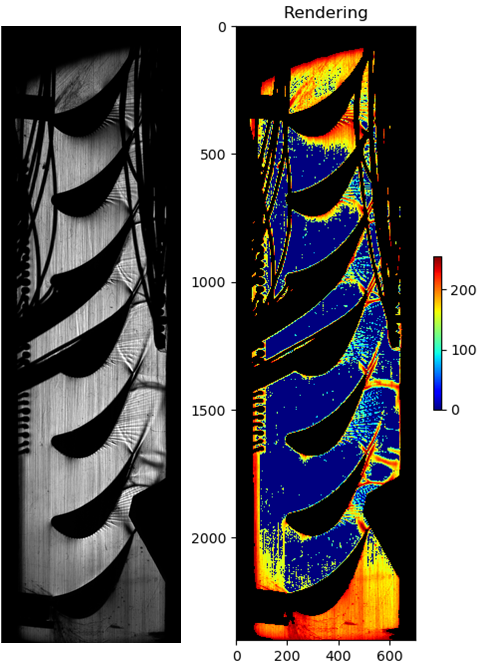
\includegraphics[width=0.75\linewidth]{src/first_show}
	\end{center}
	\caption{ \textbf{Schlieren图结果.}}
	\label{fig:first_show}	
\end{figure}
由于图像的管壁区域中存在线缆, 试件等物体, 对全图直接进行色彩映射, 会被此类区域影响; 另外, 透明管壁上由于气体流动所形成的条纹状划痕, 在图像中会呈现黑色线条噪声, 也会影响映射结果.
所以, 对流场区域分割出来,并单独进行色彩映射, 是解决问题的关键.

\paragraph{问题描述}
根据待处理的纹影图(灰度图), 我们可以将整个区域的像素分为三个像素点集: 定义Rigid为包括管壁, 试件, 线缆等区域, 记做$V_{r}$; 定义Bgk为带有大量纵向条纹噪声的透明管壁区域, 记做$V_{b}$; 定义Flow为流场区域, 记做$V_{f}$.可知

\begin{eqnarray}
	\quad &V= V_{f} \bigcup V_{r} \bigcup V_{b}\\
	\nonumber
	\quad&\forall V_i, V_j, ~~ V_i\bigcap V_j = \oslash,~~ i,j \in \{\text{r,f,b}\}&
	\label{eq:v}
\end{eqnarray}
若有掩膜(Mask)二值函数

\begin{eqnarray}
	M_{f}(p) = \left\{
		\begin{aligned}
			\quad&=&1, ~ p\in V_{f}\\
			\nonumber
			\quad&=&0, ~p \in V - V_{f}
		\end{aligned}
	\right.
	\label{eq:Mf}
\end{eqnarray}


\begin{eqnarray}
	M_{r}(p) = \left\{
		\begin{aligned}
			\quad&=&1, ~ p\in V_{r}\\
			\nonumber
			\quad&=&0, ~p \in V - V_{r}
		\end{aligned}
	\right.
	\label{eq:Mr}
\end{eqnarray}
以及

\begin{eqnarray}
	M_{b}(p) = \left\{
		\begin{aligned}
			\quad&=&1, ~ p\in V_{b}\\
			\nonumber
			\quad&=&0, ~p \in V - V_{b}
		\end{aligned}
	\right.
	\label{eq:Mb}
\end{eqnarray}



则可单独提取出各自区域像素值,如:
\begin{eqnarray}
	\nonumber
	\quad \mathop{I}\limits_{p \in V_{f}}(p)= I(p) M_{f}(p)\\
	\nonumber
	\quad \mathop{I}\limits_{p \in V_{r}}(p)= I(p) M_{r}(p)\\
	\nonumber
	\quad \mathop{I}\limits_{p \in V_{b}}(p)= I(p) M_{b}(p)
\end{eqnarray}
综上, 我们只需要对全图中各个像素进行正确分类, 则可通过分割对流场区域进行提取, 从而实现单独色彩映射.


